% !TeX program = pdflatex
\documentclass[aspectratio=169, 12pt]{beamer}
\usetheme{Madrid}
\usecolortheme{default}

% Packages for pdflatex
\usepackage[utf8]{inputenc}
\usepackage[T1]{fontenc}
\usepackage{helvet}  % Helvetica/Arial replacement for pdflatex
\usepackage{graphicx}
\usepackage{booktabs}
\usepackage{multirow}
\usepackage{array}
\usepackage{colortbl}
\usepackage{pgfplots}
\usepackage{pgf-pie}  % For pie charts
\usepackage{amsmath, amssymb}
\usepackage{tikz}
\usetikzlibrary{shapes, arrows.meta, positioning, calc}
\pgfplotsset{compat=1.18}

% Set sans-serif font as default (Helvetica looks like Arial)
\renewcommand{\familydefault}{\sfdefault}

% Custom colors
\definecolor{hkuDark}{RGB}{0, 51, 102}
\definecolor{hkuLight}{RGB}{0, 102, 153}
\definecolor{accentRed}{RGB}{204, 0, 0}
\definecolor{accentOrange}{RGB}{255, 102, 0}
\definecolor{successGreen}{RGB}{0, 153, 102}
\definecolor{warningYellow}{RGB}{255, 204, 0}

% Beamer color settings
\setbeamercolor{title}{fg=white, bg=hkuDark}
\setbeamercolor{frametitle}{fg=hkuDark}
\setbeamercolor{structure}{fg=hkuDark}
\setbeamercolor{block title}{fg=white, bg=hkuLight}
\setbeamercolor{block body}{fg=black, bg=gray!10}
\setbeamercolor{alerted text}{fg=accentRed}

% Remove navigation symbols
\setbeamertemplate{navigation symbols}{}

% Custom footer
\setbeamertemplate{footline}{
  \leavevmode%
  \hbox{%
  \begin{beamercolorbox}[wd=.333333\paperwidth,ht=2.25ex,dp=1ex,center]{date in head/foot}%
    \usebeamerfont{date in head/foot}\insertshortdate
  \end{beamercolorbox}%
  \begin{beamercolorbox}[wd=.333333\paperwidth,ht=2.25ex,dp=1ex,center]{title in head/foot}%
    \usebeamerfont{title in head/foot}IF Research @ HKU SPACE
  \end{beamercolorbox}%
  \begin{beamercolorbox}[wd=.333333\paperwidth,ht=2.25ex,dp=1ex,right]{author in head/foot}%
    \usebeamerfont{author in head/foot}\insertshortauthor\hspace*{2em}
    \insertframenumber{} / \inserttotalframenumber\hspace*{2em}
  \end{beamercolorbox}}%
  \vskip0pt%
}

% Custom title slide
\setbeamertemplate{title page}{
  \begin{center}
    \vspace{1cm}
    {\usebeamerfont{title}\usebeamercolor[fg]{title}\inserttitle\par}
    \vspace{0.5cm}
    {\usebeamerfont{subtitle}\insertsubtitle\par}
    \vspace{2cm}
    {\usebeamerfont{author}\insertauthor\par}
    \vspace{0.3cm}
    {\usebeamerfont{date}\insertdate\par}
    \vspace{0.5cm}
    \begin{center}
      \fbox{\rule{0pt}{1cm}\rule{2cm}{0pt}}
    \end{center}
  \end{center}
}

% Title info
\title{Perceptions and Experiences of Intermittent Fasting\\Among HKU SPACE Students}
\subtitle{Group Oral Presentation | English for Academic Purposes II}
\author{Member 1, Member 2, Member 3, Member 4, Member 5, Member 6}
\date{March 2026}

\begin{document}

% ==================== SLIDE 1: TITLE ====================
\begin{frame}[plain]
  \titlepage
\end{frame}

% ==================== SLIDE 2: THE PARADOX ====================
\begin{frame}{The Paradox: Popular but Unpracticed}
  \begin{center}
    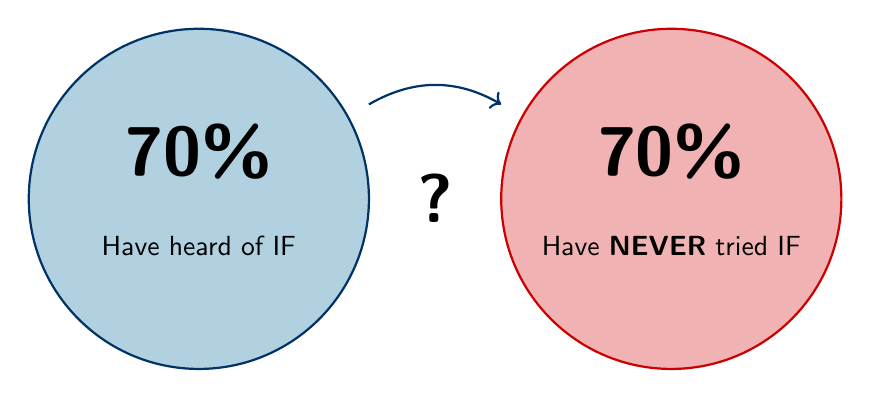
\begin{tikzpicture}[scale=1.2]
      % Left circle
      \draw[fill=hkuLight!30, draw=hkuDark, thick] (0,0) circle (1.8cm);
      \node at (0,0.5) {\Huge \textbf{70\%}};
      \node at (0,-0.5) {Have heard of IF};
      
      % Right circle
      \draw[fill=accentRed!30, draw=accentRed, thick] (5,0) circle (1.8cm);
      \node at (5,0.5) {\Huge \textbf{70\%}};
      \node at (5,-0.5) {Have \textbf{NEVER} tried IF};
      
      % Question mark
      \node at (2.5,0) {\Huge \textbf{?}};
      
      % Arrow
      \draw[->, thick, hkuDark] (1.8,1) to[out=30,in=150] (3.2,1);
    \end{tikzpicture}
  \end{center}
  \vspace{0.5cm}
  \begin{block}{Our Research Question}
    What explains the gap between awareness and action?
  \end{block}
\end{frame}

% ==================== SLIDE 3: WHAT IS IF ====================
\begin{frame}{What is Intermittent Fasting?}
  \begin{definition}[Intermittent Fasting]
    Cycling between periods of eating and fasting — focusing on \textbf{WHEN} to eat, not \textbf{WHAT} to eat.
  \end{definition}
  
  \vspace{0.5cm}
  \begin{columns}[T]
    \column{0.45\textwidth}
    \begin{block}{\textbf{16:8} Method}
      \begin{itemize}
        \item 16 hours fasting
        \item 8 hours eating window
        \item Most popular among students
      \end{itemize}
    \end{block}
    
    \column{0.45\textwidth}
    \begin{block}{\textbf{5:2} Method}
      \begin{itemize}
        \item 5 normal eating days
        \item 2 low-calorie days (500-600 kcal)
        \item Less common in our sample
      \end{itemize}
    \end{block}
  \end{columns}
  
  \vspace{0.3cm}
  \tiny \textcolor{gray}{Citation: Aragon \& Schoenfeld (2022)}
\end{frame}

% ==================== SLIDE 4: RELEVANCE ====================
\begin{frame}{Why This Matters to HKU SPACE Students}
  \begin{columns}[T]
    \column{0.5\textwidth}
    \begin{itemize}
      \item \textbf{[Schedule]} Irregular class schedules
      \item \textbf{[Study]} Academic pressure \& exams
      \item \textbf{[Meal]} Limited meal prep time
      \item \textbf{[Group]} Social pressure to eat
    \end{itemize}
    
    \column{0.5\textwidth}
    \begin{alertblock}{Top Concern from Our Data}
      \centering
      \Large \textbf{"Hunger affecting focus"}
      
      \vspace{0.3cm}
      \normalsize (Column H, Q11 — 7/30 respondents)
    \end{alertblock}
  \end{columns}
  
  \vspace{0.5cm}
  \begin{quote}
    Understanding IF in our specific student context is different from reading a clinical study.
  \end{quote}
\end{frame}

% ==================== SLIDE 5: METHODOLOGY ====================
\begin{frame}{Methodology: How We Collected Data}
  \begin{table}
    \centering
    \begin{tabular}{|l|l|}
      \hline
      \rowcolor{hkuLight!30} \textbf{Method} & Quantitative survey (online + paper) \\
      \hline
      \textbf{Sample size (N)} & 27 HKU SPACE students \\
      \hline
      \textbf{Sampling method} & Convenience (Telegram + campus) \\
      \hline
      \textbf{Time period} & March 2026 \\
      \hline
      \textbf{Analysis} & Descriptive statistics (Excel) \\
      \hline
    \end{tabular}
  \end{table}
  
  \vspace{0.5cm}
  \begin{center}
    \tiny \textcolor{gray}{Citation: Zangirolami-Raimundo et al. (2018)}
  \end{center}
\end{frame}

% ==================== SLIDE 6: DEMOGRAPHICS ====================
\begin{frame}{Who Responded? (Demographics)}
  \begin{columns}[T]
    \column{0.33\textwidth}
    \textbf{Figure 1: Gender}
    \begin{center}
      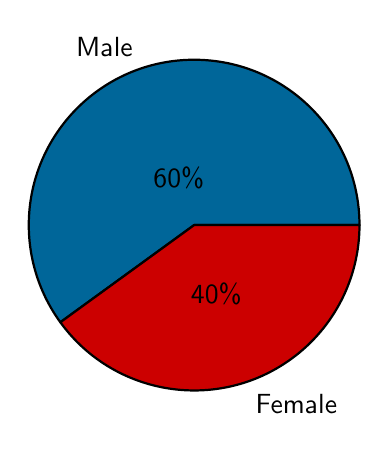
\begin{tikzpicture}[scale=0.7]
        \pie[color={hkuLight, accentRed}]{60/Male, 40/Female}
      \end{tikzpicture}
    \end{center}
    
    \column{0.33\textwidth}
    \textbf{Figure 2: BMI}
    \begin{center}
      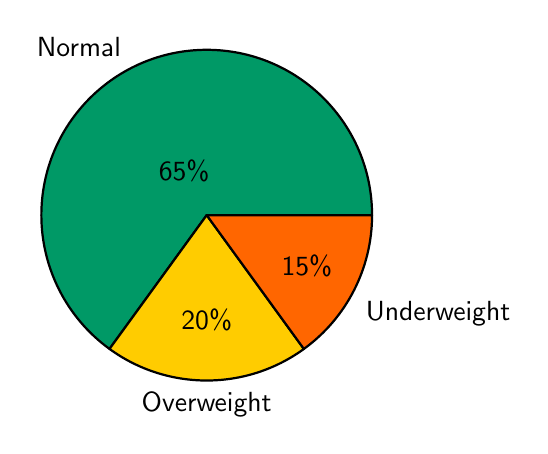
\begin{tikzpicture}[scale=0.7]
        \pie[color={successGreen, warningYellow, accentOrange}]{65/Normal, 20/Overweight, 15/Underweight}
      \end{tikzpicture}
    \end{center}
    
    \column{0.34\textwidth}
    \textbf{Figure 3: Physical Activity}
    \begin{center}
      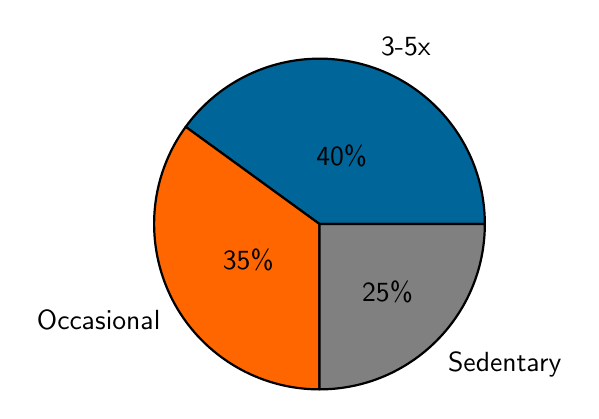
\begin{tikzpicture}[scale=0.7]
        \pie[color={hkuLight, accentOrange, gray}]{40/3-5x/week, 35/Occasional, 25/Sedentary}
      \end{tikzpicture}
    \end{center}
  \end{columns}
  
  \vspace{0.3cm}
  \begin{block}{Key Insight}
    Our respondents are already \textbf{health-conscious} — their fears about IF are genuine, not from laziness.
  \end{block}
\end{frame}

% ==================== SLIDE 7: PERCEIVED BENEFITS ====================
\begin{frame}{Perceived Benefits: Why Students Find IF Appealing}
  \begin{center}
    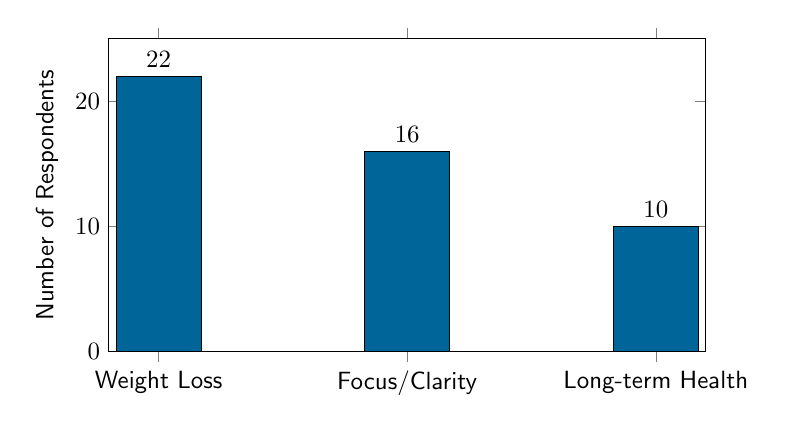
\begin{tikzpicture}[scale=0.9]
      \begin{axis}[
        ybar,
        width=10cm,
        height=6cm,
        symbolic x coords={Weight Loss, Focus/Clarity, Long-term Health},
        xtick=data,
        xticklabel style={align=center},
        ylabel=Number of Respondents,
        ymin=0,
        ymax=25,
        nodes near coords,
        bar width=1.2cm,
        ybar=2pt,
      ]
        \addplot[fill=hkuLight] coordinates {(Weight Loss, 22) (Focus/Clarity, 16) (Long-term Health, 10)};
      \end{axis}
    \end{tikzpicture}
  \end{center}
  
  \begin{alertblock}{Scientific Reality (Gudden et al., 2021)}
    \centering
    No clear evidence of short-term cognitive benefits from IF.
  \end{alertblock}
  
  \vspace{0.2cm}
  \tiny \textcolor{gray}{Data source: Column I (Q10) — Perceived benefits}
\end{frame}

% ==================== SLIDE 8: PERCEIVED RISKS ====================
\begin{frame}{Perceived Risks: What Students Fear Most}
  \begin{center}
    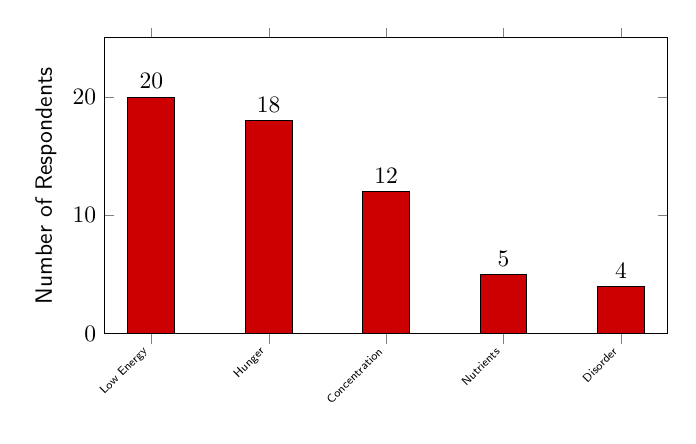
\begin{tikzpicture}[scale=0.85]
      \begin{axis}[
        ybar,
        width=10cm,
        height=6cm,
        symbolic x coords={Low Energy, Hunger, Concentration, Nutrients, Disorder},
        xtick=data,
        xticklabel style={rotate=45, anchor=east, font=\tiny},
        ylabel=Number of Respondents,
        ymin=0,
        ymax=25,
        nodes near coords,
        bar width=0.7cm,
        ybar=2pt,
      ]
        \addplot[fill=accentRed] coordinates {(Low Energy, 20) (Hunger, 18) (Concentration, 12) (Nutrients, 5) (Disorder, 4)};
      \end{axis}
    \end{tikzpicture}
  \end{center}
  
  \vspace{0.2cm}
  \begin{quote}
    "Students are less worried about long-term health risks than about surviving the next lecture without feeling faint."
  \end{quote}
  
  \tiny \textcolor{gray}{Citation: Stockman et al. (2018) — short-term trials show only marginal improvements}
\end{frame}

% ==================== SLIDE 9: INFORMATION SOURCES ====================
\begin{frame}{Where Do Students Get Information?}
  \begin{columns}[T]
    \column{0.5\textwidth}
    \begin{center}
      \textbf{Figure: Information Sources (Q6)}
      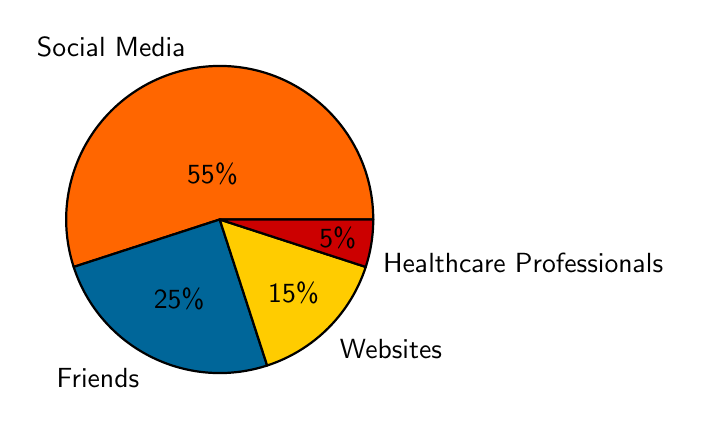
\begin{tikzpicture}[scale=0.65]
        \pie[color={accentOrange, hkuLight, warningYellow, accentRed}]{55/Social Media, 25/Friends, 15/Websites, 5/Healthcare Professionals}
      \end{tikzpicture}
    \end{center}
    
    \column{0.5\textwidth}
    \begin{alertblock}{The Problem}
      \begin{itemize}
        \item \textbf{TikTok \& Instagram} promote simple success stories
        \item \textbf{Few consult professionals}
        \item \textbf{Precision nutrition requires personalized advice}
      \end{itemize}
    \end{alertblock}
  \end{columns}
  
  \vspace{0.3cm}
  \tiny \textcolor{gray}{Citation: Soliman (2022) — Precision nutrition}
\end{frame}

% ==================== SLIDE 10: KNOWLEDGE GAP (DRAMATIC) ====================
\begin{frame}{The Critical Knowledge Gap: What Breaks a Fast?}
  \begin{center}
    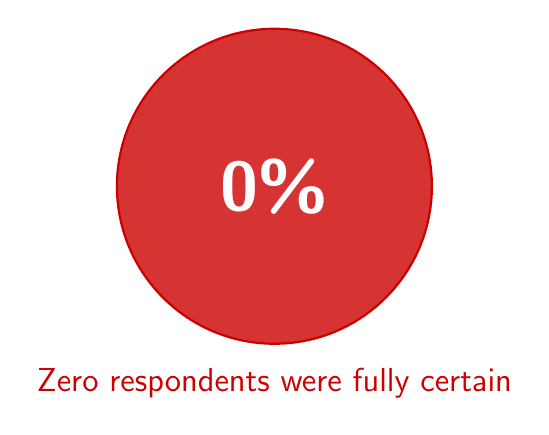
\begin{tikzpicture}
      % Dramatic 0% circle
      \draw[fill=accentRed!80, draw=accentRed, thick] (0,0) circle (2cm);
      \node at (0,0) {\Huge \textbf{\textcolor{white}{0\%}}};
      \node at (0,-2.5) {\large \textcolor{accentRed}{Zero respondents were fully certain}};
    \end{tikzpicture}
  \end{center}
  
  \vspace{0.3cm}
  \begin{columns}[T]
    \column{0.3\textwidth}
    \begin{block}{OK}
      \begin{itemize}
        \item Black coffee
        \item Unsweetened tea
        \item Water
      \end{itemize}
    \end{block}
    
    \column{0.3\textwidth}
    \begin{block}{Breaks Fast}
      \begin{itemize}
        \item Milk / Latte
        \item Sweetened drinks
        \item Diet soda (controversial)
      \end{itemize}
    \end{block}
    
    \column{0.4\textwidth}
    \begin{block}{Consequence}
      Lose metabolic benefits $\rightarrow$ Assume "IF doesn't work" $\rightarrow$ Quit
    \end{block}
  \end{columns}
  
  \tiny \textcolor{gray}{Citation: Ganesan et al. (2018) — insulin response and autophagy}
\end{frame}

% ==================== SLIDE 11: BARRIERS ====================
\begin{frame}{Barriers to Sustaining IF: The Data}
  \begin{columns}[T]
    \column{0.5\textwidth}
    \textbf{Figure 4: Greatest Impact on Maintaining IF}
    \begin{center}
      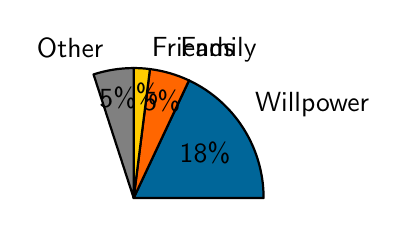
\begin{tikzpicture}[scale=0.55]
        \pie[color={hkuLight, accentOrange, warningYellow, gray}]{18/Willpower, 5/Family, 2/Friends, 5/Other}
      \end{tikzpicture}
    \end{center}
    
    \column{0.5\textwidth}
    \textbf{Figure 5: Biggest Student Barriers}
    \begin{center}
      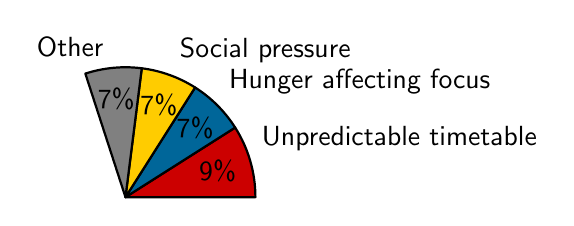
\begin{tikzpicture}[scale=0.55]
        \pie[color={accentRed, hkuLight, warningYellow, gray}]{9/Unpredictable timetable, 7/Hunger affecting focus, 7/Social pressure, 7/Other}
      \end{tikzpicture}
    \end{center}
  \end{columns}
  
  \vspace{0.3cm}
  \begin{block}{Conclusion}
    IF fails not because students lack discipline, but because \textbf{student life is fundamentally unpredictable}.
  \end{block}
  
  \tiny \textcolor{gray}{Citation: Lin et al. (2025) — adherence challenges in early vs. late time-restricted eating}
\end{frame}

% ==================== SLIDE 12: SUMMARY OF FINDINGS ====================
\begin{frame}{Summary of Key Findings}
  \begin{enumerate}
    \item \textbf{Perception-Reality Gap:} Students see IF as effective for weight loss and focus, but science has not confirmed short-term cognitive benefits.
    \pause
    \item \textbf{Information Crisis:} \textcolor{accentRed}{Social media} is the main source — not healthcare professionals.
    \pause
    \item \textbf{Knowledge Void:} \textcolor{accentRed}{Zero} students fully understand what breaks a fast.
    \pause
    \item \textbf{Structural Barriers:} Unpredictable schedules and social pressure are real obstacles, not laziness.
  \end{enumerate}
  
  \vspace{0.5cm}
  \begin{center}
    \large \textcolor{hkuDark}{A cycle of failed attempts and abandoned diets.}
  \end{center}
\end{frame}

% ==================== SLIDE 13: RECOMMENDATION 1 ====================
\begin{frame}{Recommendation 1: Improve Nutritional Literacy}
  \begin{block}{\large What HKU SPACE Can Do}
    \begin{itemize}
      \item \textbf{Post clear guidelines} near vending machines:
      \begin{quote}
        "Black coffee = OK. Latte = Breaks fast."
      \end{quote}
      \item \textbf{Promote trusted websites} (not TikTok) for IF information
      \item \textbf{Emphasize protein-rich foods} during eating windows:
      \begin{itemize}
        \item Meat, fish, eggs, legumes
      \end{itemize}
    \end{itemize}
  \end{block}
  
  \vspace{0.3cm}
  \tiny \textcolor{gray}{Citation: Ganesan et al. (2018)}
\end{frame}

% ==================== SLIDE 14: RECOMMENDATION 2 ====================
\begin{frame}{Recommendation 2: Adapt IF to Academic Life}
  \begin{block}{\large Student Strategies}
    \begin{enumerate}
      \item \textbf{Match eating windows to your lecture schedule}
      \begin{itemize}
        \item Late class $\rightarrow$ shift eating window later
      \end{itemize}
      \item \textbf{Use appetite suppressants:} Black coffee or green tea during study sessions
      \item \textbf{Prepare high-protein portable snacks:}
      \begin{itemize}
        \item Hard-boiled eggs, whole wheat sandwiches
      \end{itemize}
      \item \textbf{Discuss goals with friends/family} to reduce social pressure
    \end{enumerate}
  \end{block}
  
  \vspace{0.3cm}
  \begin{center}
    \large \textcolor{successGreen}{IF must fit your life, not the other way around.}
  \end{center}
  
  \tiny \textcolor{gray}{Citation: Johnstone (2015)}
\end{frame}

% ==================== SLIDE 15: CONCLUSION ====================
\begin{frame}{Conclusion: Key Takeaways}
  \begin{center}
    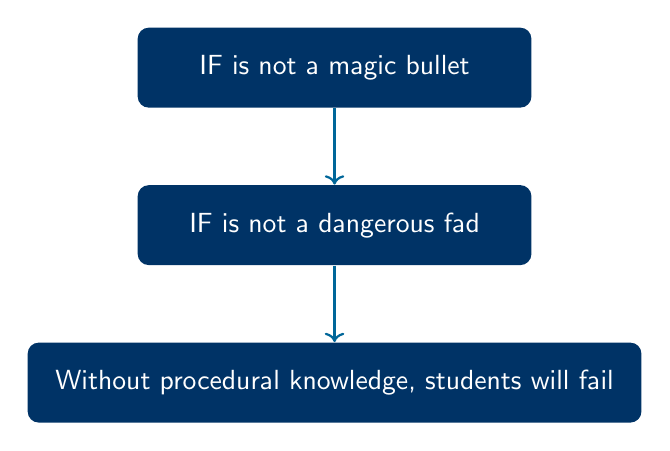
\begin{tikzpicture}
      \node[fill=hkuDark, text=white, rounded corners, inner sep=10pt, minimum width=5cm] (box1) at (0,2) {IF is not a magic bullet};
      \node[fill=hkuDark, text=white, rounded corners, inner sep=10pt, minimum width=5cm] (box2) at (0,0) {IF is not a dangerous fad};
      \node[fill=hkuDark, text=white, rounded corners, inner sep=10pt, minimum width=5cm] (box3) at (0,-2) {Without procedural knowledge, students will fail};
      
      \draw[->, thick, hkuLight] (box1) -- (box2);
      \draw[->, thick, hkuLight] (box2) -- (box3);
    \end{tikzpicture}
  \end{center}
  
  \vspace{0.5cm}
  \begin{center}
    \Large \textbf{Information + Adaptation = Sustainable IF}
  \end{center}
  
  \vspace{0.3cm}
  \begin{quote}
    "HKU SPACE can play a small but important role by providing clear, evidence-based guidance."
  \end{quote}
\end{frame}

% ==================== SLIDE 16: Q&A / REFERENCES ====================
\begin{frame}{Questions?}
  \begin{center}
    \Huge \textbf{Thank you for listening.}
    
    \vspace{1cm}
    \Large Any questions?
    
    \vspace{1.5cm}
    \normalsize \textbf{References:}
    \begin{columns}[T]
      \column{0.5\textwidth}
      \tiny
      \begin{itemize}
        \item Aragon \& Schoenfeld (2022). \textit{Nutritional timing revisited.}
        \item Ganesan et al. (2018). \textit{Intermittent fasting: A review.}
        \item Gudden et al. (2021). \textit{The effects of IF on cognition.}
        \item Johnstone (2015). \textit{Fasting for weight loss.}
      \end{itemize}
      
      \column{0.5\textwidth}
      \tiny
      \begin{itemize}
        \item Lin et al. (2025). \textit{Adherence challenges in TRE.}
        \item Soliman (2022). \textit{Precision nutrition.}
        \item Stockman et al. (2018). \textit{Intermittent fasting for obesity.}
        \item Zangirolami-Raimundo et al. (2018). \textit{Survey methodology.}
      \end{itemize}
    \end{columns}
  \end{center}
\end{frame}

% ==================== END ====================
\end{document}
